\documentclass[conference]{IEEEtran}
\IEEEoverridecommandlockouts
\usepackage{cite}
\usepackage[utf8]{inputenc}
\usepackage{newunicodechar}
\newunicodechar{∼}{\textasciitilde}
\usepackage{amsmath}
\usepackage{amssymb}
\usepackage{booktabs}
\usepackage{graphicx}
\graphicspath{{./}}
\usepackage{tikz}
\usetikzlibrary{positioning,arrows.meta}
\usepackage{pifont}
\usepackage{enumitem}
\usepackage{url}
\usepackage{xcolor}
\newcommand{\cmark}{\ding{51}}\newcommand{\xmark}{\ding{55}}
\newcommand{\rs}[1]{\textcolor{green!55!black}{[RS: #1]}}
\newcommand{\ba}[1]{\textcolor{orange}{[BA: #1]}}

\begin{document}

\title{Beyond Designed Signatures: Learning Compact Polygon Signatures for
Weighted Jaccard Similarity Search}
% Alternative titles for review:
% (1) Learned Signatures for Compact Polygon Shape-Similarity Search
% (3) Learning Compact Shape Signatures for Large-Scale Polygon Similarity Search
%     via Weighted Jaccard Distillation
% (4) Small Learned Signatures for Large Polygon Collections: Distilling Weighted
%     Jaccard Similarity
% (previous) Weighted-Jaccard-Native Distillation for Compact Polygon Similarity
%     Search under Extreme Area Variation

\author{\IEEEauthorblockN{1\textsuperscript{st} Ruban Sampath}
\IEEEauthorblockA{\textit{Department of Computer Science} \\
\textit{University of Texas at San Antonio}\\
San Antonio, TX, USA \\
ruban.s@utsa.edu}
\and
\IEEEauthorblockN{2\textsuperscript{nd} Buddhi Ashan M. K.}
\IEEEauthorblockA{\textit{Department of Computer Science} \\
\textit{University of Texas at San Antonio}\\
San Antonio, TX, USA \\
buddhiashan.mallikakankanamalage@utsa.edu}
\and
\IEEEauthorblockN{3\textsuperscript{rd} Sushil K. Prasad}
\IEEEauthorblockA{\textit{Department of Computer Science} \\
\textit{University of Texas at San Antonio}\\
San Antonio, TX, USA \\
sushil.prasad@utsa.edu}
}

\maketitle

\begin{abstract}
Finding polygons with similar shapes in large geospatial datasets underlies map
conflation, land-use change detection, and geospatial intelligence. Here, shape
similarity is defined as area intersection independent of location, for which the Jaccard
index, the ratio of intersection to union area, is the standard metric. The
state-of-the-art, ShapeToVec, handles datasets consisting of polygon
areas spanning many orders of magnitude by encoding each polygon on an adaptive
quadtree grid as a high-dimensional floating-point vector. The Weighted Jaccard (WJ)
similarity between these vectors, the generalization of Jaccard to nonnegative
vectors, approximates the polygons' Jaccard index and can be searched directly using
an index. This accuracy comes at a high cost in memory and query throughput.
ShapeToVec+ compresses these vectors into bit signatures up
to $32\times$ smaller, but loses substantial accuracy at its most aggressive
settings, with recall@50 falling from $96\%$ to $76\%$. Both methods rely on
\emph{designed} signatures: hand-engineered encodings with no learned component. We
introduce \emph{learned} signatures, obtained by distilling ShapeToVec vectors into a
compact encoder whose outputs lie on the probability simplex and are compared
directly under WJ. \ba{Add one explaining the architecture in one line as it is listed as a contribution.}
It is a two-layer multilayer perceptron whose final normalization makes every
output entry nonnegative and sum to one.
\rs{Done} The encoder is trained with a listwise ranking loss that
supervises each polygon's exact top-$k$ most similar shapes rather than individual
similarity values, and it outperforms alternative training objectives at every width
we test. Because it is trained Matryoshka-style, a single training run yields one
encoder that serves every width from 256 to 4096 dimensions by simple truncation. \ba{Above sentence does not read well.}\rs{Done} On
the Parks dataset with 233K polygons, our signatures are up to $47\times$ smaller
than ShapeToVec vectors, exceeding ShapeToVec+'s compression, while reaching $92\%$
recall@50 without reranking, within $5$ points of ShapeToVec's best and well above
ShapeToVec+'s $76\%$, at up to $14\times$ its throughput. With a lightweight exact
reranking step, they surpass ShapeToVec's best recall while remaining
${\sim}3\times$ faster than its most accurate configuration.
\end{abstract}

\begin{IEEEkeywords}
polygon similarity search, weighted Jaccard, listwise ranking loss, metric distillation, approximate nearest neighbor, probability simplex
\end{IEEEkeywords}

\section{Introduction}
\label{sec:intro}
% \ba{Please put the content for the following sub-sections to build the
% Introduction properly. In general, no need to add numbers unless they are
% core. No need to cite sections, equations etc. Add paper citations as
% needed.}\rs{Done -- content added below under each subsection; internal
% section/equation references removed throughout, numbers trimmed to the ones that
% felt load-bearing. Titles left in for this review pass, to strip later per your
% note.}

% \subsection{Motivation}

% \ba{Too long. Please split into multiple sentences.}\rs{Done -- split up.}
% \ba{The above paragraph does not read well. Please check}\rs{Done -- rewritten with
% smoother transitions; added why compactness matters at today's dataset sizes.}
Finding similar shapes in large polygon datasets is a fundamental geospatial
operation, supporting tasks from deduplication and map conflation to geospatial
intelligence. In environmental monitoring, for instance, tracking how a lake shrinks
or an ice shelf fragments over time requires matching each new observation against
its closest-shaped counterpart in a large historical archive~\cite{shape2vec}. These
collections now reach hundreds of millions of polygons~\cite{shapetovecplus26}. At
that scale, how compactly each polygon is represented decides whether similarity
search fits in memory at all. For instance,  floating-point encodings of 90 million polygons already
exceed a terabyte of memory~\cite{shapetovecplus26}.

% \subsection{Problem Statement}

Shape-similarity retrieval is defined as: given a query polygon, return the
polygons that are most similar to its shape, independent of the location in a large database of polygons. The Jaccard
similarity, the ratio of
intersection to union area between two polygons, is the standard measure of this
similarity. Computing this similarity score requires expensive geometric intersection
against every candidate, where practical systems instead encode each polygon as a vector
over a shared spatial grid and compare the vectors employing Weighted Jaccard
(WJ) metric~\cite{rajaraman11}. A core challenge in solving this problem is that real-world
polygon areas vary by many orders of magnitude, and no single, uniform grid
resolution serves both regimes at once: a grid fine enough to resolve small polygons
explodes in dimension when applied to large ones, while a grid coarse enough to stay
tractable collapses small polygons into near-empty, uninformative vectors. Serving
both regimes accurately therefore pushes encodings to high dimension, which is what
makes search at scale costly.

% \subsection{State of the Art and Limitations}

Early polygon-encoding approaches, including Fourier
descriptors~\cite{ai13fourier} and graph convolutional
autoencoders~\cite{yan21gcae}, target building datasets with narrow, comparable
shape categories. However, over real-world datasets, where polygon areas span many orders of
magnitude, they retrieve similar shapes poorly~\cite{shape2vec}, since neither
representation was designed to preserve that scale of area variation.

ShapeToVec~\cite{shape2vec} addresses this gap by employing an adaptive quadtree grid that recursively subdivides
space where polygon detail is concentrated, encoding each polygon as a
high-dimensional floating-point feature vector. Subsequently, a Hierarchical Navigable Small World (HNSW)
graph~\cite{hnsw20} is constructed over the polygon encodings under a custom WJ distance, maintaining high accuracy. However, its high-dimensional floating-point vectors do not scale well, as storing and searching them grows expensive as a dataset grows.

ShapeToVec+~\cite{shapetovecplus26} improves scalability while maintaining high accuracy. This is achieved by decoupling the true area values from the feature vectors into an occupancy level. The produced small signatures, which only track the occupancy level, recover the true area at query time from a pre-built lookup table which stores individual cell area values of the quadtree nodes. This allows ShapeToVec's raw floating-point cell values
into signatures up to $32\times$ smaller. However, with the bit encoding, which is the most aggressive
setting, the occupancy signature is too coarse to distinguish between small and large occupancy levels, leading to substantially degraded accuracy. 
% Both methods remain
% \emph{designed} signatures: fixed, hand-engineered encoding rules with no learned
% component, and therefore neither can adapt its footprint to what actually matters
% for a given collection's shapes.
% \ba{On the paragraph above: Bring the 'designed' nature of this work at the
% beginning. Emphasize its ability to decouple cell area into a lookup table and
% encoding to only indicate cell area overlap level.}\rs{Done -- opens with
% ``designed'' now and explains the lookup-table decoupling mechanism.}

Matryoshka representation
learning~\cite{matryoshka22} is a widely adopted technique for multi-width
embeddings under Euclidean and cosine similarity. It trains a single embedding whose
leading prefixes stay useful at every truncation width, letting one model serve many
deployment sizes. It has not been applied to polygon geometries or to WJ. We adopt its truncation method, even though the
representation itself does not produce WJ-compatible embeddings.
% \ba{'so' is not suitable for technical writing. Explain related building dataset
% papers with autoencoders and Fourier Transformers and mention they did not work
% well with this data and explain briefly why. Why do you mention this
% representation specifically, as it has not been used with geometries before? Is
% this SOTA for the distances mentioned? Please specify why you mention this.}\rs{Done
% -- Fourier/autoencoder prior art moved to the start of this subsection, with
% evidence for why they fail; Matryoshka now has its own paragraph, described as the
% widely adopted multi-width technique for Euclidean/cosine retrieval, never applied
% to geometries, and mentioned because we reuse its truncation idea.}

% \subsection{Closing the Gap}

% \ba{The limitation that we fill is to achieve aggressive compression through learned
% signatures, leading to improved scalability and efficiency. We should not say we
% just tried learned and it worked.}\rs{Done -- opens by naming the compression
% ceiling designed signatures hit, then frames learned signatures as removing it.}
A designed signature compresses
every cell by the same fixed rule, regardless of how much that cell helps
distinguish shapes in a given collection, and accuracy therefore drops once
compression is pushed far. A learned signature removes this ceiling. Rather than hand-engineering a fixed encoding
rule, we train an encoder directly on the ground-truth shape similarity structure,
allowing it to capture what makes two polygons similar in shape and represent that information
as compactly, improving scalability and query efficiency beyond
what designed signatures permit. Instead of shrinking each dimension's precision, we learn a much
smaller set of new dimensions that jointly preserve the similarity ranking.

% \subsection{Proposed Approach}

% \ba{Explain encoder briefly. What is new here?}\rs{Done -- names the architecture
% and states explicitly that the network itself is standard; what is new is the
% training objective.}
Our encoder is a compact neural network, a two-layer multilayer perceptron, that
maps each feature vector to a smaller vector representation. A final
normalization makes every output entry nonnegative and the entries sum to one,
placing the output on the probability simplex. This makes the compact vectors
directly comparable under WJ metric, and they are searched with the same HNSW index
ShapeToVec uses.
Our encoder follows a standard architecture, but our
training employs
a listwise ranking loss that supervises each polygon's exact top-$k$ most similar
shapes rather than individual similarity values. The compact signatures thus learn
to reproduce the ranking that retrieval depends on. The same training run also
covers every embedding width: applying the loss to nested prefixes of the output,
Matryoshka-style, lets one encoder serve any width by truncation. \ba{The above sentence does not look to fit here.}\rs{Done} At query time, a lightweight exact reranking step over
the candidate set returned by HNSW, and then exceeds, ShapeToVec's
uncompressed recall. \ba{For comparison, we should also do reranking in ShapeToVec and see?}

% \subsection{Contributions}

Our contributions are as follows:
\begin{itemize}
  \item 
  % \ba{Rephrase the description according to what I sent in discord.}\rs{Done --
  %   reframed around the ShapeToVec $\to$ ShapeToVec+ $\to$ us story from Discord.}
    \textbf{Learned signatures that exceed current compression ceiling at
    on-par or better accuracy.} To our knowledge, these are the first learned,
    shape-aware signatures for WJ polygon retrieval, and they move past the
    $32\times$ ceiling of ShapeToVec+'s designed signatures. Against ShapeToVec's own
    published results~\cite{shape2vec} on the identical Parks dataset, our embeddings
    are up to $47\times$ smaller than their tested configurations. Without
    reranking, they stay within a few points of
    ShapeToVec's recall and well above ShapeToVec+'s at its $32\times$ setting; with a
    lightweight exact reranking step, they exceed ShapeToVec's recall at several-fold
    its throughput.
  \item 
  % \ba{Write directly describe the feature you have.}\rs{Done -- reworded to lead
  %   with the feature.}
    \textbf{A rank-aware listwise loss that makes the training objective the retrieval
    metric itself.} WJ-native distillation trains the compressed embedding's own
    ranking to match the ground-truth WJ ranking directly, rather than regressing its
    absolute value. It outperforms absolute-value regression (MSE) and five further
    alternative objectives at every scale we test.
  \item 
  % \ba{Present the contribution as you did in contribution 1 and then
  %   explain.}\rs{Done -- headline claim first, explanation after.}
    \textbf{A single learned encoder that serves every width in its trained range.}
    One model serves every embedding width from 256 to 4096 dimensions by
    truncation, with no retraining per width. The range itself is a training-time
    configuration, not a fixed
    architectural choice: a different range, such as widths below 256, needs no
    redesign, only a new training run over that range. Among the widths we test, 256
    dimensions gives the best recall--throughput trade-off.
\end{itemize}

\section{Related Work}
\label{sec:related}
For two polygons encoded as non-negative vectors $\mathbf{a},\mathbf{b}\in\mathbb{R}^D_{\ge0}$
over a shared partition of $D$ spatial cells, where $a_i$ is polygon $\mathbf{a}$'s
area-weighted occupancy of cell $i$, Weighted Jaccard is
\begin{equation}
  WJ(\mathbf{a},\mathbf{b}) = \frac{\sum_i \min(a_i,b_i)}{\sum_i \max(a_i,b_i)},
  \quad \mathbf{a},\mathbf{b} \ge \mathbf{0}.
  \label{eq:wj}
\end{equation}

\textbf{ShapeToVec and its gap.} ShapeToVec~\cite{shape2vec} is the state of the art
for WJ polygon retrieval: its adaptive quadtree grid encodes each polygon as a
high-dimensional floating-point vector, and a custom Weighted Jaccard
distance it adds to NMSLIB~\cite{boytsov13} lets HNSW index these vectors directly,
reaching $97\%$ R@50 (versus $67\%$ for its binary bit-vector variant). That accuracy,
however, rests on tens of thousands of dimensions: ShapeToVec itself notes that such
vectors strain HNSW memory as datasets grow, and that generic compression
(e.g.\ product quantization~\cite{jegou10pq}) shrinks the footprint only by
\emph{degrading} accuracy. A follow-up, ShapeToVec+~\cite{shapetovecplus26}, targets
this directly with two encoding families: 8-bit integer signatures that match
float32 accuracy at $4\times$ compression, and 1--4-bit signatures that reach
$8\times$--$32\times$ compression at a real accuracy cost, down to $76\%$ recall at
their most aggressive ($32\times$) setting versus float32's $96\%$ on the identical
dataset. Both remain \emph{exact} computations over the same quadtree encoding, with
no learned component.
We fill this gap with a learned, WJ-native compression, up to $72\times$ smaller than
the raw $D{\approx}18{,}382$ input, that comes within a few points of ShapeToVec's own
reported accuracy uncompressed, and exceeds it after a cheap exact-WJ rerank pass
(\S\ref{sec:exp}).
WJ \emph{sketching} (ICWS~\cite{ioffe10}, ProbMinHash~\cite{probminhash20},
PolyMinHash~\cite{polyminhash25}) gives unbiased estimators but integer codes
incompatible with float-vector approximate-nearest-neighbor (ANN) indexes. Learned
hashing~\cite{hashsurvey14,deephashsurvey22} and Matryoshka representation
learning~\cite{matryoshka22} target Hamming/cosine spaces and degrade on the WJ
simplex (Table~\ref{tab:results}); NMF~\cite{nmf99} gives simplex factors but
optimises reconstruction, not retrieval. Knowledge distillation~\cite{hinton15}
transfers a teacher's outputs to a student; we adapt it to a \emph{metric},
distilling exact WJ into a compact simplex embedding; none of the above target
WJ as the native metric.

\textbf{Ranking objectives vs.\ value regression.} Learning-to-rank losses such as
RankNet~\cite{burges05} (pairwise) and ListNet~\cite{cao07} (listwise) are a
further alternative to the margin-based contrastive losses of
\S\ref{sec:contrastive}: rather than pushing a single hardest negative below a
margin, they optimise pairwise or listwise order directly, which could plausibly
avoid the margin loss's collapse at scale (\S\ref{sec:contrastive}) without giving
up on matching the deployed metric the way pure value regression does. We test
this directly (\S\ref{sec:distill}): a ListNet-style listwise objective, applied to
our WJ-native setting, beats absolute-value MSE regression by a wide, consistent
margin at every scale (10K/512-d R@50 $0.973$ vs.\ $0.930$; 50K/256-d R@50 $0.921$
vs.\ $0.794$; 233K/256-d R@50 $0.906$ vs.\ $0.797$), unlike the pairwise/margin
losses of \S\ref{sec:contrastive}, which do collapse at scale. The distinguishing
factor is not ``ranking vs.\ value'' as a category: it is whether the training
target is \emph{graded} (proportional to true similarity, as both MSE and listwise
targets are here) or \emph{binary} (positive/negative, as our earlier triplet and
InfoNCE targets are) -- a graded softmax target lets listwise both match the
deployed metric's full similarity structure per anchor \emph{and} directly optimise
the ranking recall depends on. We additionally implemented and tested five further
rank-aware and Matryoshka-training refinements: four sourced from 2025--2026
literature (sequential/curriculum Matryoshka training, cross-batch hard-negative
memory, and learnable dimension selection, all from~\cite{smec25}; cross-dimension
self-distillation~\cite{mipic26}), and a fifth, an angle-wise geometric relational
term, drawing on the older (2019) RKD formulation~\cite{park19rkd} rather than a new
one; none improved on plain listwise, and three actively hurt retrieval quality (full
results and mechanistic analysis in
our released code and logs, \S\ref{sec:exp}). We report this not to claim
listwise is unimprovable, but because a compact WJ embedding's loss function
deserves a justified choice rather than an assumed one, given how many rank-aware
alternatives the recent literature now offers.

\section{Method}
\label{sec:method}
\ba{Above is already mentioned in the abstract and intro. Not see the value for stating again.}\rs{Done.}
Our method has two
phases (Fig.~\ref{fig:pipeline}).
\ba{Replace 'parts' with 'phases' throughout the paper.}\rs{Done.}
An encoder maps each vector to a compact embedding
that can be searched directly under WJ distance.
\ba{It has to be WJ distance throughout the paper.}\rs{Done.}
A listwise distillation loss trains the
encoder to reproduce the neighbor ranking given by exact WJ on the original vectors,
at several embedding widths at once.
\ba{I think this paragraph can explain the overview of the encoder and training process can be excluded from here.}\rs{Done.}

\begin{figure}[t]\centering
\resizebox{\columnwidth}{!}{%
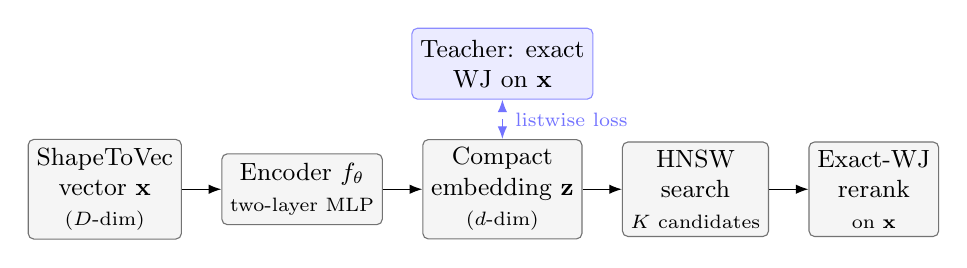
\begin{tikzpicture}[font=\small,>={Latex[length=1.6mm,width=1.2mm]},
  node distance=4.5mm and 5mm,
  box/.style={draw=black!55,rounded corners=2pt,fill=black!4,
              minimum height=9mm,align=center,inner sep=3pt},
  tbox/.style={box,fill=blue!8,draw=blue!45}]
 \node[box] (x) {ShapeToVec\\vector $\mathbf{x}$\\{\scriptsize ($D$-dim)}};
 \node[box,right=of x] (e) {Encoder $f_\theta$\\{\scriptsize two-layer MLP}};
 \node[box,right=of e] (z) {Compact\\embedding $\mathbf{z}$\\{\scriptsize ($d$-dim)}};
 \node[tbox,above=5mm of z] (t) {Teacher: exact\\WJ on $\mathbf{x}$};
 \node[box,right=of z] (h) {HNSW\\search\\{\scriptsize $K$ candidates}};
 \node[box,right=of h] (r) {Exact-WJ\\rerank\\{\scriptsize on $\mathbf{x}$}};
 \draw[->](x)--(e); \draw[->](e)--(z);
 \draw[<->,dashed,blue!55](z)--node[right=0.4mm]{\scriptsize listwise loss}(t);
 \draw[->](z)--(h); \draw[->](h)--(r);
\end{tikzpicture}}
\caption{Overview. The encoder maps a polygon's float32 vector to a compact
embedding whose entries are nonnegative and sum to one. During training (dashed), a
listwise loss aligns the embedding's WJ ranking with the exact WJ ranking of the
original vectors. At query time, HNSW retrieves $K$ candidates using the compact
embeddings, and exact WJ on the original vectors re-sorts them. \ba{As mentioned before, you can call float32 vectors or something instead ShapeToVec vec}\rs{Done.}}
\label{fig:pipeline}
\end{figure}

\subsection{Problem Setup}
\label{sec:setup}
Each polygon is represented by its ShapeToVec vector
$\mathbf{x}\in\mathbb{R}^{D}_{\ge0}$. Entry $x_i$ is the polygon's area-weighted
occupancy of cell $i$ in ShapeToVec's adaptive quadtree grid~\cite{shape2vec}, and
$D$ is the number of grid cells ($D\approx18$K for Parks). These vectors are sparse:
about $73\%$ of their entries are zero. We call the WJ between two original vectors
(Eq.~\ref{eq:wj}) the \emph{teacher similarity}. Given a corpus of polygons, we learn
an encoder $f_\theta$ that maps each $\mathbf{x}$ to an embedding
$\mathbf{z}=f_\theta(\mathbf{x})$ of width $d\ll D$. The goal is to preserve rankings.
For a query polygon, sorting the corpus by the WJ between embeddings should place the
same polygons at the top as sorting by the teacher similarity. Exact similarity values
matter only insofar as they determine this order. The encoder is trained on corpus
polygons only; all queries are held out.

\subsection{Encoder}
\label{sec:embed}
Before encoding, we divide each ShapeToVec vector by the sum of its entries. The raw
sums span many orders of magnitude, mirroring the area variation of the polygons
themselves, and normalization places every input on a common scale. The teacher
similarity is still computed on the original, unnormalized vectors.

The encoder is a two-layer multilayer perceptron (MLP). Each layer applies a linear
map, then batch normalization~\cite{ioffe15bn}, then a ReLU. Both layers have 4096
units, for about 92M parameters in total. Three design choices follow from the
nature of the input.

\noindent\textbf{Why an MLP.} The input is already a fixed-length vector over a grid
shared by all polygons, and an MLP maps it directly to a fixed-length output. Neural
polygon encoders in the literature instead consume raw geometry: Transformers over
boundary points~\cite{mai22}, graph networks over vertices~\cite{polygongnn24}, and
set encoders~\cite{deepsets17}. Using them would discard the quadtree encoding that
makes ShapeToVec robust to area variation. They are also trained for Euclidean or
cosine similarity, not WJ.

\noindent\textbf{A dense first layer.} The first layer connects every grid cell to
every hidden unit. Each hidden unit can therefore combine cells from anywhere in the
grid, such as cells that tend to be occupied together. This layer holds about 75M of
the 92M parameters.

\noindent\textbf{Batch normalization before ReLU.} Because most input entries are
zero, many pre-activations sit near zero, and a ReLU applied directly could leave
many units inactive. Batch normalization re-centers and rescales each unit before
the ReLU, which helps keep units active on these sparse inputs.

\subsection{Output Normalization}
\label{sec:simplex}
WJ is defined for nonnegative vectors. The encoder's final ReLU makes every output
entry nonnegative, and dividing by the sum makes the entries sum to one. Writing
$h_\theta$ for the MLP,
\begin{equation}
  f_\theta(\mathbf{x}) = \frac{\mathrm{ReLU}(h_\theta(\mathbf{x}))}
       {\max(\|\mathrm{ReLU}(h_\theta(\mathbf{x}))\|_1,\;\epsilon)},
  \label{eq:simplex}
\end{equation}
where $\|\cdot\|_1$ is the sum of absolute entries and $\epsilon$ is a small
constant that avoids division by zero. A vector with nonnegative entries that sum to
one lies on the \emph{probability simplex}. This is the only sense in which we use
the term, and it describes our embeddings, not the ShapeToVec input. Normalizing has
two benefits. First, every embedding has the same total mass, and WJ then compares
how that mass is distributed across entries rather than how large it is. Second,
for two such vectors WJ has a closed form in their $\ell_1$ distance,
$WJ(\mathbf{z},\mathbf{z}')=(2-\|\mathbf{z}-\mathbf{z}'\|_1)/(2+\|\mathbf{z}-\mathbf{z}'\|_1)$,
which makes computing all pairwise similarities in a training batch fast. The
embeddings are indexed with the same WJ distance that ShapeToVec added to
NMSLIB~\cite{shape2vec,boytsov13}, with no post-processing.

\subsection{Training Objective: Listwise WJ Distillation}
\label{sec:distill}
We train the encoder by \emph{distillation}~\cite{hinton15}, in which a compact
student learns to reproduce the outputs of a more expensive teacher. Here the student
is the encoder, and the teacher is not a network but the exact WJ between original
vectors. What the student must reproduce is the ranking this teacher induces.

\noindent\textbf{Training batches.} Before training, we find each corpus polygon's
$P$ most similar corpus polygons by exact search over the normalized input vectors
($P{=}30$ at the 50K and full-dataset scales). Each training batch samples 512
polygon--neighbor (anchor--positive) pairs, giving $N{=}1024$ polygons. A batch therefore contains a few
highly similar pairs and many pairs of unrelated polygons. As
Fig.~\ref{fig:batchdist} shows, the teacher similarities of the unrelated pairs are
spread out rather than concentrated at zero. Each polygon's row of similarities thus
carries graded information beyond its one paired neighbor.

\noindent\textbf{Loss.} For polygons $i$ and $j$ in a batch, let $T_{ij}$ be their
teacher similarity and $\hat T_{ij}$ the WJ between their embeddings. For each
polygon $i$, a softmax with temperature $\tau$ turns its row of teacher similarities
into a probability distribution $p_i$ over the other polygons in the batch. The same
operation on the embedding similarities gives $\hat p_i$. The loss is the
cross-entropy between the two, averaged over the batch:
\begin{align}
  p_{ij}&=\frac{\exp(T_{ij}/\tau)}{\sum_{k\neq i}\exp(T_{ik}/\tau)},\quad
  \hat p_{ij}=\frac{\exp(\hat T_{ij}/\tau)}{\sum_{k\neq i}\exp(\hat T_{ik}/\tau)},\notag\\
  \mathcal{L}_{\mathrm{list}}&=-\frac{1}{N}\sum_i\sum_{j\neq i} p_{ij}\log\hat p_{ij}.
  \label{eq:distill}
\end{align}
We use $\tau=0.1$. At this temperature the teacher distribution places most of its
weight on each polygon's most similar batch members. The loss is lowest when the
embedding ranks the same polygons at the top, in the same order, as the teacher,
which is what recall@$k$ measures. This formulation follows the listwise
learning-to-rank approach of ListNet~\cite{cao07}.

\noindent\textbf{Why not match similarity values directly.} The simplest distillation
loss is the mean squared error (MSE) between $\hat T_{ij}$ and $T_{ij}$ over all
pairs. MSE spends equal effort on every pair, including the many low-similarity pairs
that never appear in a top-$k$ result. It also rewards reproducing each value rather
than reproducing the order. The listwise loss concentrates on the order at the top of
each row. With architecture, data, and training budget held fixed, it improves
recall@50 over MSE by 4 to 13 points at every scale we test
(Table~\ref{tab:lossablation}). Five further refinements from recent literature,
layered on top of the listwise loss, did not improve on it
(Section~\ref{sec:related}).

\begin{table}[t]\centering
\caption{Loss comparison: recall@50 before reranking. Architecture, data, and
training budget are identical; only the loss differs. $\ddagger$~=~ours.}
\label{tab:lossablation}\small\setlength{\tabcolsep}{5pt}
\begin{tabular}{@{}lrrr@{}}
\toprule
Scale (dim) & MSE R@50 & Listwise R@50$^\ddagger$ & $\Delta$ \\
\midrule
10K (512-d)  & 0.930 & \textbf{0.973} & $+4.3$\,pp \\
50K (256-d)  & 0.794 & \textbf{0.921} & $+12.6$\,pp \\
233K (256-d) & 0.797 & \textbf{0.906} & $+10.9$\,pp \\
\bottomrule
\end{tabular}
\end{table}

\begin{figure}[t]\centering
\includegraphics[width=0.85\columnwidth]{fig_batch_wj_dist.png}
\caption{Teacher similarities $T_{ij}$ within one training batch (10K), split into
sampled anchor--positive pairs and all remaining pairs in the batch. The remaining
pairs are broadly spread, not concentrated at zero.}
\label{fig:batchdist}
\end{figure}

\subsection{One Encoder for Many Widths}
\label{sec:matryoshka}
Following Matryoshka representation learning~\cite{matryoshka22}, one encoder serves
several widths. During training, the loss in Eq.~\eqref{eq:distill} is computed on
the first $m$ entries of each embedding, renormalized to sum to one, for every
$m\in\{256,512,1024,2048,4096\}$, and the five losses are averaged. The leading
entries are thereby trained to be useful on their own. At deployment, choosing a
width means keeping the first $d$ entries and renormalizing, with no retraining. The
set of widths is a training setting, not part of the architecture. A different
range, such as widths below 256, needs a new training run but no change to the
model. Within the trained range, recall is nearly flat from 256 to 4096 dimensions
(Section~\ref{sec:exp}), which makes 256 the natural operating point.

Sharing one encoder across widths has a small cost. Compared with encoders trained
for a single width under the same architecture, data, and budget, the shared encoder
loses about 1.1 to 1.2 points of recall@50 before reranking, at both 256 and 4096
dimensions. The 4096-dimensional case involves no truncation, which indicates that
the cost comes from the five losses competing during training, not from truncation.
Reranking reduces the difference to within noise. We accept this cost in exchange for
a single trained model that covers every operating point.

\subsection{Two-Stage Retrieval}
\label{sec:twostage}
Search runs in two stages. In the first stage, an HNSW index~\cite{hnsw20} over the
compact embeddings, using ShapeToVec's WJ distance, returns $K$ candidates for a
query. In the second stage, we compute exact WJ between the query's original vector
and each candidate's original vector, and re-sort the candidates. The HNSW index
stores only the compact embeddings. The original vectors are accessed only for each
query's $K$ candidates. The second stage can reorder candidates but cannot add new
ones. The value of $K$ therefore sets the trade-off between speed and recall: a
larger $K$ costs more time but is more likely to contain the true top-$k$ neighbors.
A good embedding lets a small $K$ contain them. We use $K{=}2000$ and the same HNSW
settings throughout ($M{=}20$; efConstruction and efSearch both $200$). Results
labeled Stage-1 use the first stage alone.

\subsection{Contrastive Alternatives}
\label{sec:contrastive}
We compare against contrastive objectives widely used to train retrieval embeddings,
applied to the same encoder with WJ as the similarity. A \emph{triplet}
loss~\cite{schroff15} requires each polygon to be more similar to a true neighbor
than to the most similar non-neighbor in the batch, by a fixed margin. A batch can
contain other true neighbors of the same polygon, and a \emph{false-negative filter}
excludes these before the hardest non-neighbor is chosen. \emph{InfoNCE}~\cite{oord18}
also applies a softmax over the batch, but its target places all weight on the one
paired neighbor. Variants add a decoder reconstruction term or a WJ regression term
(Table~\ref{tab:ablation}). All of these objectives use binary targets: a pair is
either a neighbor or not. They push neighbors above non-neighbors but say nothing
about the order among neighbors, or among the rest of the corpus. The listwise loss
instead uses graded targets taken from the teacher similarity itself. This
difference matters at scale. The contrastive models perform reasonably at 10K but fall
to the level of an untrained random projection at 50K, while distillation does not
(Section~\ref{sec:exp}).

\subsection{Two-stage retrieval}
\label{sec:twostage}
Stage-1 builds an HNSW index ($M{=}20$, $\mathrm{ef}{=}200$)~\cite{hnsw20} under
ShapeToVec's custom Weighted Jaccard distance~\cite{shape2vec} over the $d$-dim
embeddings and retrieves a candidate pool of size $K$ per query; Stage-2 reranks
only that pool by exact WJ on the original $D$-dim vectors (Numba~\cite{lam15}),
recovering near-exact ordering within it. Because Stage-2 can only reorder the pool
Stage-1 hands it, not enlarge it, $K$ is the single knob that trades recall for
speed end to end: a larger $K$ costs more HNSW and rerank time but is more likely to
contain the true top-$k$ neighbours; the compact embedding's job is to make a
\emph{small} $K$ already contain them.

\section{Experiments}
\label{sec:exp}
We use the publicly released ShapeToVec dataset~\cite{shapetovec-data}: quadtree
encodings and shape-similarity ground truth for the Parks polygons (233{,}773;
originally OpenStreetMap~\cite{osm} data, distributed via the SpatialHadoop
benchmark~\cite{eldawy15}), at its highest-fidelity resolution
($D{=}18{,}382$ dimensions for the 50K benchmark, ${\sim}18.2$--$18.5$k across
subsets), the finest, costliest-to-index resolution and so the most valuable to
compress. The main benchmark is a 50K set partitioned into a 40k-polygon \emph{corpus}
(the indexed database that queries are searched against) and 10k held-out query
polygons; we also use a 10k subset (8k corpus / 2k queries) for the moderate-scale
study and the full 233k Parks dataset (187,019-polygon corpus / 46{,}754 queries) for
a scaling check. At 50k and 233k, learned methods are \emph{corpus-trained}: trained only on
corpus-internal neighbour pairs, so every query is held out and the numbers measure
generalization to unseen queries; at 10k they are trained on the 2k-query set. Ground
truth is the exact \emph{geometric} (shapely) Jaccard on the polygon geometry;
ShapeToVec's own validation shows the quadtree-vector WJ tracks this closely (RMSE
$10.16\%$ at $K{=}50$, $11.84\%$ at $K{=}500$, stable across grid
resolutions)~\cite{shape2vec}. We report R@$k$ ($k\in\{10,50,500\}$) and QPS (PyTorch~\cite{paszke19},
AdamW~\cite{loshchilov19}, cosine annealing~\cite{loshchilov17}). All runs use an
NVIDIA DGX~A100 (8$\times$ A100-SXM4 80\,GB GPUs, dual 64-core AMD EPYC~7742 CPUs,
2\,TB RAM); QPS is measured on a single GPU. \footnote{Code, trained models, and
evaluation scripts: \url{https://github.com/ruban-ai/polygon-ann-ml-embeddings}.}

\begin{table}[t]\centering
\caption{Stage-1 recall on the 10k subset (no rerank). $\dagger$~brute-force.
\textbf{Bold}~=~best ANN method; $\ddagger$~=~ours.}
\label{tab:results}\setlength{\tabcolsep}{4pt}\small
\begin{tabular}{@{}llrrrr@{}}
\toprule
Method & Dim & R@10 & R@50 & R@500 & QPS \\
\midrule
PCA~\cite{jolliffe02}                   & 512  & 0.432 & 0.553 & 0.789 & 16{,}666 \\
NMF~\cite{nmf99}                        & 512  & 0.638 & 0.727 & 0.942 & 11{,}764 \\
Rand.\ Proj.~\cite{achlioptas03}        & 512  & 0.687 & 0.759 & 0.930 &  9{,}663 \\
ICWS~\cite{ioffe10}$^\dagger$           & 512  & 0.840 & 0.897 & 0.988 &     139 \\
Matryoshka MLP~\cite{matryoshka22}      & 512  & 0.455 & 0.672 & 0.932 & 18{,}647 \\
\addlinespace[2pt]
MLP WJ-triplet$^\ddagger$               & 512  & 0.677 & 0.806 & 0.964 & 10{,}756 \\
InfoNCE--WJ$^\ddagger$                  & 512  & 0.490 & 0.698 & 0.947 &  7{,}160 \\
AE WJ-tri+recon$^\ddagger$              & 512  & 0.711 & 0.858 & 0.977 & 10{,}903 \\
MSE distill$^\ddagger$        & 512  & 0.844 & 0.930 & 0.994 & 14{,}552 \\
\textbf{Listwise distill}$^\ddagger$ & \textbf{512} & \textbf{0.945} & \textbf{0.973} & \textbf{0.996} & \textbf{9{,}690} \\
\bottomrule
\end{tabular}
\end{table}

\textbf{Moderate scale (Table~\ref{tab:results}).}
WJ-distillation is the strongest method regardless of loss choice, and the listwise
variant is stronger still: R@50 $=0.973$, $+4.3$\,pp over MSE distillation and
$+11.5$\,pp over the best contrastive model, above brute-force ICWS (0.897) at
${\sim}70\times$ its throughput. Reranking lifts R@10 above $0.996$ for all
variants (not shown).

\textbf{The 50K benchmark (Table~\ref{tab:full50k}).}
On 40k corpus polygons with 10k fully held-out queries, the contrastive methods
collapse to the level of an untrained random projection: triplet and InfoNCE reach
only Stage-1 R@500 $\approx 0.72$, at or below random projection ($0.77$--$0.84$
across dimensions). WJ-distillation, by aligning objective and metric, reaches
R@500 $=0.969$ at 256-d (listwise; MSE reaches only $0.924$ at the same width, see
Table~\ref{tab:lossablation}), and after reranking delivers the highest recall at
competitive throughput: R@500 $=0.990$ at 1{,}083 QPS. Even at its best dimension
(4096-d), random projection reaches only $0.972$ reranked, still below
distillation's 256-d $0.990$. To our knowledge,
this is the first learned WJ embedding to beat random projection on \emph{both} the
near- and wide-net frontiers.

\textbf{Compression versus ShapeToVec's own published results (Table~\ref{tab:uncompressed}).}
Every comparison above is against \emph{other compressed} representations (random
projection, contrastive baselines, MSE distillation). ShapeToVec's own paper~\cite{shape2vec}
reports results at their tested resolutions ($3$k, $6$k, and $12$k dimensions) directly
on the Parks dataset (233,773 polygons, the same 80/20 corpus/query split we use
throughout), giving a genuine same-dataset reference point. At their best (12k-d),
floating-point ShapeToVec vectors indexed under HNSW reach Recall@50 $=97\%$ at $359$
QPS; at their smallest tested (3k-d), $96\%$ at $1{,}263$ QPS. Our Matryoshka encoder, at
every width we test ($256$--$4096$-d, all at or below their largest tested
resolution), reaches Recall@50 $=92.1$--$92.9\%$ without any reranking, within
$3$--$5$pp of their best published recall, at $4$--$14\times$ the throughput. Our
256-d embedding is $47\times$ smaller than their 12k-d vectors and ${\sim}12\times$
smaller than their 3k-d vectors; the ``up to $47\times$'' figure quoted elsewhere is
this best-case comparison against their highest-resolution configuration. A single,
cheap exact-WJ rerank
pass over the retrieved candidates closes and exceeds that gap: our 256-d embedding
reaches Recall@50 $=99.7\%$ after reranking, exceeding ShapeToVec's own best published
number, while remaining ${\sim}3\times$ faster than their most accurate (12k-d)
configuration.

\begin{table}[t]\centering
\caption{Our compressed embeddings vs.\ ShapeToVec's own published
results~\cite{shape2vec} (Table III there, floating-point encoding), identical Parks
dataset (233,773 polygons, same 80/20 corpus/query split), Recall@50, no rerank, sorted
by dimension. $\ddagger$~=~ours.}
\label{tab:uncompressed}\setlength{\tabcolsep}{4pt}\small
\begin{tabular}{@{}lrr@{}}
\toprule
Method (dim) & R@50 & QPS \\
\midrule
Ours, 256-d$^\ddagger$  & 92.1\% & 4{,}921 \\
Ours, 512-d$^\ddagger$  & 92.5\% & 2{,}682 \\
Ours, 1024-d$^\ddagger$ & 92.8\% & 1{,}958 \\
Ours, 2048-d$^\ddagger$ & 92.9\% & 1{,}631 \\
ShapeToVec, ${\sim}3$k-d & 96\% & 1{,}263 \\
Ours, 4096-d$^\ddagger$ & 92.9\% & 1{,}493 \\
ShapeToVec, ${\sim}6$k-d & 96\% & 735 \\
ShapeToVec, ${\sim}12$k-d & 97\% & 359 \\
\bottomrule
\end{tabular}
\end{table}

\textbf{Recall by polygon class (Table~\ref{tab:bucket}).} The paper's motivating
claim is that extreme area variation is the hard case (\S\ref{sec:intro}), so we
break the 50K benchmark's Stage-1 recall down by query-polygon area quartile (Q1 =
smallest 25\% of the 10k held-out queries by encoded area, Q4 = largest) and,
separately, by quadtree-cell count (a shape-complexity proxy; same pattern, omitted
for space). WJ-distillation (listwise) is essentially flat across the size range
(R@50 $0.918$--$0.927$), while random projection degrades sharply on large
polygons: R@50 falls from $0.753$ at Q1 to $0.594$ at Q4, a $16$pp gap absent from
distillation. The compact embedding does not merely match random projection on
average, as Table~\ref{tab:full50k} shows; it is uniform across exactly the axis of
variation ShapeToVec was built to handle, where the untrained baseline is not, and
listwise is if anything flatter than MSE was at this same breakdown (MSE R@50 range
was $0.784$--$0.801$, 1.7\,pp; listwise's is $0.9$\,pp).

\begin{table}[t]\centering
\caption{Stage-1 recall by polygon-area quartile (50K benchmark, listwise, 256-d,
no rerank). Q1 = smallest 25\% of held-out queries by encoded area, Q4 = largest.
$\ddagger$~=~ours.}
\label{tab:bucket}\setlength{\tabcolsep}{3pt}\footnotesize
\begin{tabular}{@{}lrrrr@{}}
\toprule
Quartile & Distill R@50$^\ddagger$ & Distill R@500$^\ddagger$ & RP R@50 & RP R@500 \\
\midrule
Q1 (smallest) & 0.927 & 0.975 & 0.753 & 0.854 \\
Q2             & 0.920 & 0.963 & 0.661 & 0.729 \\
Q3             & 0.918 & 0.963 & 0.637 & 0.734 \\
Q4 (largest)   & 0.919 & \textbf{0.977} & 0.594 & 0.776 \\
\bottomrule
\end{tabular}
\end{table}

\textbf{Why contrastive fails (Fig.~\ref{fig:layer}).}
The collapse is due to objective--metric misalignment, not capacity limit. Within a
trained contrastive model, Stage-1 recall \emph{rises} the further a layer sits from
the loss: the deployed output is the \emph{worst} layer (R@500 $0.65$, below random
projection's $0.77$), while an untouched intermediate layer is best ($0.82$). Rank
fidelity mirrors this: the Spearman correlation between embedding-WJ and true-WJ
falls from $0.76$ at that layer to $0.14$ at the output, so the loss harms exactly
the representation it is meant to produce.

\begin{figure}[t]\centering
\includegraphics[width=0.74\columnwidth]{fig_layer_tap.png}
\caption{The contrastive loss damages the layer it is applied to. Within one trained
contrastive model, Stage-1 recall \emph{falls} the closer the layer is to the loss:
the deployed 512-d output is the \emph{worst} layer, below an untrained random
projection, while an untouched intermediate layer is best.}
\label{fig:layer}
\end{figure}

\textbf{The full Parks dataset (Table~\ref{tab:full233}).}
Our WJ-distillation encoder, with identical architecture, loss, and 256-d prefix as on
the 50K benchmark, scales unchanged to the full 233k Parks dataset: trained only on
corpus neighbours and evaluated on \emph{all} 46{,}754 held-out queries, listwise
reaches Stage-1 R@500 $=0.946$ and $0.982$ after reranking, versus MSE's $0.890$ and
$0.966$ at the same width -- the listwise-over-MSE margin established at 10K/50K
(Table~\ref{tab:lossablation}) holds at the largest scale we test too.

\begin{table}[t]\centering
\caption{The full 233k Parks dataset: WJ-distillation (listwise) on \emph{all}
46{,}754 held-out queries (187,019-polygon corpus-trained), 256-d prefix. MSE row shown
for comparison (Table~\ref{tab:lossablation}).}
\label{tab:full233}\setlength{\tabcolsep}{4pt}\small
\begin{tabular}{@{}lrrrr@{}}
\toprule
Stage & R@10 & R@50 & R@500 & QPS \\
\midrule
Stage-1, MSE (no rerank)        & 0.720 & 0.797 & 0.890 & 2{,}136 \\
Stage-1, listwise (no rerank)   & 0.862 & 0.906 & 0.946 & 2{,}538 \\
\textbf{+ exact-WJ rerank (listwise)} & \textbf{0.993} & \textbf{0.996} & \textbf{0.982} & 1{,}065 \\
\bottomrule
\end{tabular}
\end{table}

\begin{table}[t]\centering
\caption{50K benchmark (40k corpus / 10k held-out queries; geometric-Jaccard GT).
All methods corpus-trained, shown at 256-d. $\ddagger$~=~ours. \textbf{Bold}~=~best.}
\label{tab:full50k}\setlength{\tabcolsep}{3.5pt}\small
\begin{tabular}{@{}llrrrr@{}}
\toprule
Method & $K$ & R@10 & R@50 & R@500 & QPS \\
\midrule
\multicolumn{6}{@{}l@{}}{\textit{Stage 1 --- no rerank}}\\[1pt]
Rand.\ Proj.~\cite{achlioptas03}    & --- & 0.616 & 0.659 & 0.766 & 3{,}890 \\
triplet+recon$^\ddagger$            & --- & 0.494 & 0.600 & 0.725 & 3{,}810 \\
InfoNCE--WJ$^\ddagger$              & --- & 0.459 & 0.560 & 0.720 & 7{,}128 \\
MSE distill$^\ddagger$       & --- & 0.692 & 0.794 & 0.924 & 6{,}772 \\
\textbf{Listwise distill}$^\ddagger$ & --- & \textbf{0.871} & \textbf{0.921} & \textbf{0.969} & \textbf{4{,}921} \\
\midrule
\multicolumn{6}{@{}l@{}}{\textit{Stage 2 --- exact-WJ rerank}}\\[1pt]
Rand.\ Proj.~\cite{achlioptas03}    & 2000 & 0.994 & 0.995 & 0.955 & 904 \\
triplet+recon$^\ddagger$            & 2000 & 0.994 & 0.994 & 0.859 & 898 \\
InfoNCE--WJ$^\ddagger$              & 2000 & 0.993 & 0.987 & 0.821 & 1{,}345 \\
MSE distill$^\ddagger$       & 2000 & 0.995 & 0.997 & 0.976 & 1{,}253 \\
\textbf{Listwise distill}$^\ddagger$ & 2000 & \textbf{0.995} & \textbf{0.997} & \textbf{0.990} & \textbf{1{,}083} \\
\bottomrule
\end{tabular}
\end{table}

\textbf{A second polygon class: water bodies (Table~\ref{tab:wb50k}).} Every result
so far is on Parks; to test whether WJ-distillation is Parks-specific we build an
identically-scaled benchmark (40k corpus / 10k held-out queries, methodology
matching \S\ref{sec:exp}) on the SpatialHadoop water-body
collection~\cite{eldawy15}, with the same architecture, loss, and 256-d prefix,
no method changes. The gap over random projection is, if anything, larger than on
Parks: Stage-1 R@50 $=0.912$ vs.\ $0.632$ ($+28.0$pp) and R@500 $=0.965$ vs.\
$0.763$ ($+20.2$pp), at higher throughput ($6{,}293$ vs.\ $2{,}652$ QPS) --
both the recall margin and the listwise-over-MSE margin established on Parks
(MSE reaches only R@50 $=0.815$, R@500 $=0.930$ here) hold on this second polygon
class. After reranking, distillation's 256-d reaches R@500 $=0.994$ at $1{,}300$
QPS ($K{=}2000$), versus random projection's best dimension (4096-d) reaching only
$0.971$ at $246$ QPS, the same pattern as the Parks 50K benchmark
(\S\ref{sec:exp}). WJ-native distillation is not tuned to one polygon class.

\begin{table}[t]\centering
\caption{Water-body benchmark (40k corpus / 10k held-out queries; same
methodology as the Parks 50K benchmark), shown at 256-d. $\ddagger$~=~ours.
\textbf{Bold}~=~best.}
\label{tab:wb50k}\setlength{\tabcolsep}{3.5pt}\small
\begin{tabular}{@{}llrrrr@{}}
\toprule
Method & $K$ & R@10 & R@50 & R@500 & QPS \\
\midrule
\multicolumn{6}{@{}l@{}}{\textit{Stage 1 --- no rerank}}\\[1pt]
Rand.\ Proj.~\cite{achlioptas03}    & --- & 0.563 & 0.632 & 0.763 & 2{,}652 \\
MSE distill$^\ddagger$       & --- & 0.722 & 0.815 & 0.930 & 4{,}632 \\
\textbf{Listwise distill}$^\ddagger$ & --- & \textbf{0.858} & \textbf{0.912} & \textbf{0.965} & \textbf{6{,}293} \\
\midrule
\multicolumn{6}{@{}l@{}}{\textit{Stage 2 --- exact-WJ rerank}}\\[1pt]
Rand.\ Proj.~\cite{achlioptas03}    & 2000 & 0.994 & 0.994 & 0.958 & 362 \\
MSE distill$^\ddagger$       & 2000 & 0.995 & 0.997 & 0.987 & 1{,}280 \\
\textbf{Listwise distill}$^\ddagger$ & 2000 & \textbf{0.995} & \textbf{0.997} & \textbf{0.994} & \textbf{1{,}300} \\
\bottomrule
\end{tabular}
\end{table}

\textbf{The full water-body dataset (Table~\ref{tab:wbfull}).} To confirm the 50K
water-body result is not a small-scale artifact, we repeat the full-scale protocol of
Table~\ref{tab:full233} on the complete 448,550-polygon water-body collection
(ShapeToVec's own reported size for this dataset~\cite{shape2vec}): corpus-trained on
all 358,840 corpus polygons, evaluated on \emph{all} 89,710 held-out queries.
Listwise reaches Stage-1 R@50 $=0.899$, R@500 $=0.944$, and R@500 $=0.992$ after
reranking, versus MSE's R@50 $=0.815$, R@500 $=0.898$ at the same width -- the
listwise-over-MSE margin holds at this scale and on this second polygon class too.
Against ShapeToVec's own published water-body numbers on the identical dataset
($96$--$97\%$ R@50 at $3$k--$12$k-d), our embeddings show a wider pre-rerank gap here
than on Parks ($89.9$--$91.8\%$ R@50, $5$--$7$pp behind, versus Parks' $3$--$5$pp) and
the throughput advantage is not uniform: our largest width ($4096$-d, $702$ QPS) is
slower than their smallest ($3$k-d, $1{,}036$ QPS). The same cheap exact-WJ rerank
pass again closes and exceeds the gap regardless: 256-d reaches R@50 $=99.5\%$ at
$789$ QPS, still ${\sim}2.7\times$ faster than ShapeToVec's most accurate (12k-d)
configuration. WJ-native distillation generalizes to this harder second polygon class
with a real but bounded pre-rerank cost, fully recovered after reranking.

\begin{table}[t]\centering
\caption{The full 448,550-polygon water-body dataset: WJ-distillation (listwise) on
\emph{all} 89,710 held-out queries (358,840-polygon corpus-trained), 256-d prefix.
MSE row shown for comparison.}
\label{tab:wbfull}\setlength{\tabcolsep}{4pt}\small`
\begin{tabular}{@{}lrrrr@{}}
\toprule
Stage & R@10 & R@50 & R@500 & QPS \\
\midrule
Stage-1, MSE (no rerank)        & 0.745 & 0.815 & 0.898 & 1{,}654 \\
Stage-1, listwise (no rerank)   & 0.855 & 0.899 & 0.944 & 2{,}039 \\
\textbf{+ exact-WJ rerank (listwise)} & \textbf{0.993} & \textbf{0.995} & \textbf{0.992} & 789 \\
\bottomrule
\end{tabular}
\end{table}

\textbf{Trade-off between dimension and throughput (Fig.~\ref{fig:dim}, Table~\ref{tab:dim}).}
Because the encoder is Matryoshka, one model serves every width. Listwise
distillation's recall is essentially flat from 256 to 4096 (R@500
$0.969\!\to\!0.973$) while QPS falls ${\sim}3.3\times$, so 256-d, a $72\times$
compression versus the raw input, is the natural operating point: it is the narrowest
width we test at which recall is still statistically indistinguishable from the
widest, so there is no accuracy reason to deploy anything larger, and it is where we
stop testing narrower widths too -- the width range is a training-time configuration
rather than an architectural limit (\S\ref{sec:intro}), so a floor below 256-d is a
natural next experiment, not something this curve rules out. Baselines, by contrast, stay below
distillation at \emph{every} width. This gentler QPS decay is also why listwise's
throughput advantage over MSE distillation (Table~\ref{tab:lossablation}) is
dimension-dependent rather than uniform: MSE's throughput falls ${\sim}7\times$ from
256-d to 4096-d against listwise's ${\sim}3.3\times$, so MSE is faster at small widths
(256--1024-d) but the two cross over by 2048-d, where listwise pulls ahead
($1{,}631$ vs.\ $1{,}180$ QPS) and stays ahead at 4096-d ($1{,}493$ vs.\ $967$). Since
listwise's loss supervises relative order rather than absolute magnitude, we conjecture
it packs useful signal into a lower \emph{effective} dimensionality even at large
nominal widths, letting its search cost grow more slowly with $d$; we have not verified
this directly (e.g.\ via an effective-rank measurement) and note it as a plausible
explanation rather than a demonstrated mechanism.

\begin{figure}[t]\centering
\includegraphics[width=0.86\columnwidth]{fig_dim_distill.png}
\caption{WJ-distillation (listwise) on the 50K benchmark: Stage-1 recall is flat
across dimension while HNSW throughput rises sharply at small $d$; 256-d is the
sweet spot.}
\label{fig:dim}
\end{figure}

\begin{table}[t]\centering
\caption{50K Stage-1 recall vs.\ dimension (40k corpus, 10k held-out queries).
Distillation is one Matryoshka model truncated per row; baselines shown for
contrast (256\,/\,4096). Listwise's 256-d row is identical to
Table~\ref{tab:full50k} and omitted here to avoid repeating it.
$\ddagger$~=~ours.}
\label{tab:dim}\setlength{\tabcolsep}{3pt}\footnotesize
\begin{tabular}{@{}lrrrr@{}}
\toprule
Method ($d$) & R@10 & R@50 & R@500 & QPS \\
\midrule
triplet+recon$^\ddagger$ & 0.494\,/\,0.495 & 0.600\,/\,0.601 & 0.725\,/\,0.734 & 3810\,/\,710 \\
InfoNCE$^\ddagger$       & 0.459\,/\,0.464 & 0.560\,/\,0.563 & 0.720\,/\,0.720 & 7128\,/\,1168 \\
Rand.\ Proj.             & 0.616\,/\,0.705 & 0.659\,/\,0.749 & 0.766\,/\,0.841 & 3890\,/\,704 \\
Distill (MSE)$^\ddagger$ & 0.692\,/\,0.693 & 0.794\,/\,0.796 & 0.924\,/\,0.925 & 6772\,/\,967 \\
\addlinespace[2pt]
\textbf{Distill} 512$^\ddagger$ & 0.877 & 0.925 & 0.971 & 2{,}682 \\
\textbf{Distill} 1024$^\ddagger$ & 0.880 & 0.928 & 0.972 & 1{,}958 \\
\textbf{Distill} 2048$^\ddagger$ & 0.881 & 0.929 & 0.973 & 1{,}631 \\
\textbf{Distill} 4096$^\ddagger$ & 0.881 & 0.929 & 0.973 & 1{,}493 \\
\bottomrule
\end{tabular}
\end{table}

\textbf{Ablation (Table~\ref{tab:ablation}).} On 10k, the false-negative
filter is essential: adding WJ regression \emph{without} it collapses recall to
R@10 $=0.510$, while with it recall is restored (R@50 $0.808$); decoder
reconstruction then adds $+5.0$\,pp R@50 (to $0.858$).

\begin{table}[t]\centering
\caption{Component ablation (Stage-1, 10k, no rerank). The FN filter and decoder
reconstruction are both required; without filtering, WJ regression collapses.}
\label{tab:ablation}\small\setlength{\tabcolsep}{4pt}
\begin{tabular}{@{}llcrr@{}}
\toprule
Model & FN filter & Aux.\ loss & R@10 & R@50 \\
\midrule
MLP & \xmark & ---           & 0.677 & 0.806 \\
MLP & \cmark & ---           & 0.656 & 0.773 \\
MLP & \xmark & WJ regression & 0.510 & 0.736 \\
MLP & \cmark & WJ regression & 0.669 & 0.808 \\
AE  & ---    & recon.\ only  & 0.665 & 0.745 \\
\textbf{AE} & \cmark & \textbf{triplet+recon} & \textbf{0.711} & \textbf{0.858} \\
\bottomrule
\end{tabular}
\end{table}

\section{Conclusion}
We compress ShapeToVec WJ vectors up to $47\times$ with a WJ-native simplex embedding.
Against ShapeToVec's own published results on the identical Parks dataset, our
compact embeddings reach within a few points of their best recall without any
reranking, at several-fold higher throughput, and exceed it entirely after a cheap
exact-WJ rerank pass, while remaining several-fold faster than their most accurate
configuration. Contrastive objectives work at moderate scale but collapse to
random-projection level at 50K, since they optimise separation rather than the WJ
ranking recall needs. WJ-native distillation removes this misalignment, and a
rank-aware \emph{listwise} formulation of it beats absolute-value regression
decisively at every scale we test (10K/50K/233K) and against five further
rank-aware alternatives: a single Matryoshka encoder beats random projection and a
brute-force sketch estimator at both near- and wide-net recall, confirmed up to 233k
polygons and on a second polygon class. Future work targets billion-scale corpora and
other simplex-embeddable set metrics.

\section*{Acknowledgment}
Claude (Anthropic) assisted with debugging and manuscript formatting. 
Research support: NSF award \#2313039.

\bibliographystyle{IEEEtran}
\bibliography{refs}

\end{document}
